\documentclass[11pt,a4paper]{article}

% --- Packages ---
\usepackage[utf8]{inputenc}
\usepackage[T1]{fontenc}
\usepackage{amsmath,amssymb,amsthm}
\usepackage{mathtools}
\usepackage{booktabs}
\usepackage{graphicx}
\usepackage[colorlinks=true,citecolor=blue,linkcolor=blue,urlcolor=blue]{hyperref}
\usepackage{geometry}
\usepackage{setspace}
\usepackage[expansion=false,protrusion=false]{microtype}
\usepackage{tikz}
\usetikzlibrary{shapes,arrows,positioning,fit,calc}
\usepackage{xcolor}

\definecolor{codeblue}{RGB}{0,102,204}
\definecolor{darkgreen}{RGB}{0,128,0}

\newtheorem{theorem}{Theorem}[section]
\newtheorem{definition}{Definition}[section]
\newtheorem{proposition}{Proposition}[section]

% --- Page geometry ---
\geometry{
  top=1in,
  bottom=1in,
  left=1.1in,
  right=1.1in,
}

\setstretch{1.08}

% --- Title ---
\title{
  \vspace{-1.5cm}
  \textbf{Cerdic: Private, Leveraged FX on Arc}
  \vspace{-0.3cm}
}

\author{
  Cerdic Protocol Contributors\\[4pt]
  \texttt{https://cerdic.org}
}

\date{}

\begin{document}

\maketitle
\thispagestyle{empty}

\vspace{0.3cm}

\begin{abstract}
  \noindent Circle's Arc blockchain settles stablecoin value with sub-second finality and USDC-native gas, and Circle's own StableFX engine now settles \emph{spot} FX conversion between stablecoins on Arc~\cite{circlearc, circle_stablefx}. Neither provides \emph{leveraged} FX exposure, and neither hides who is trading what. Cerdic is the layer above that: a clearing kernel that lets a trader post collateral once and open margined FX, crypto, and RWA positions against it, matched privately through a trusted execution environment (TEE) rather than a public order book. This paper describes the kernel, the portfolio margin model that makes leverage capital-efficient, the TEE matching design that makes it private, and where Cerdic sits relative to existing onchain perpetuals (Ostium) and Arc's own settlement infrastructure (StableFX).
\end{abstract}

\vspace{0.3cm}

\noindent\textbf{Keywords:} portfolio margin, leverage, FX derivatives, TEE, private matching, stablecoin settlement

\newpage
\tableofcontents
\newpage

%=============================================================================
\section{Introduction}
\label{sec:introduction}
%=============================================================================

Arc is a stablecoin-native chain: deterministic sub-second finality, USDC as native gas, EVM compatibility~\cite{circlearc, arc_technical}. In late 2025 Circle added StableFX, an RFQ engine that settles spot stablecoin-to-stablecoin FX conversion directly on Arc with payment-versus-payment finality~\cite{circle_stablefx}. Between Arc and StableFX, the settlement problem for stablecoin FX is solved.

What is missing is leverage and privacy. StableFX converts EURC to USDC at spot; it does not let a treasury hedge a EURC receivable with a margined FX forward, and every conversion it settles is visible onchain. A firm managing FX risk at size does not want its hedge ratio, timing, or currency exposure legible to anyone watching the chain.

\textbf{Cerdic} is a clearing kernel and margin engine that sits above Arc's settlement layer. It does three things:

\begin{enumerate}
  \item \textbf{Portfolio margin.} Collateral is posted once, against the whole account, not per position. A long EURC/USDC hedge can net against a USDC-denominated perpetual instead of each requiring its own margin.
  \item \textbf{Private matching.} Orders are matched inside a TEE, not a public mempool or visible order book. The chain sees a settled trade; it does not see the order that produced it.
  \item \textbf{Yield-bearing collateral.} Collateral sitting behind a position earns yield (USYC and similar instruments) instead of sitting idle.
\end{enumerate}

FX is the first market because it is the one Arc's own roadmap is explicit about, and because Ostium already shows there is real demand for onchain leveraged FX/RWA exposure~\cite{ostium} -- just not privately, and not with portfolio margin. Section~\ref{sec:related} compares Cerdic to both StableFX and Ostium directly.

\subsection{What this paper covers}

Section~\ref{sec:related} places Cerdic against StableFX and Ostium concretely. Section~\ref{sec:model} defines actors and threat model. Section~\ref{sec:architecture} gives the layered design. Section~\ref{sec:clearing} is the clearing kernel; Section~\ref{sec:margin} is the portfolio margin formula and liquidation logic. Section~\ref{sec:markets} covers the market extension interface and the FX module specifically. Section~\ref{sec:privacy} is the TEE matching design. Section~\ref{sec:agents} and~\ref{sec:yield} cover agent accounts and yield-bearing collateral. Section~\ref{sec:economics} is the fee model. Section~\ref{sec:security} is a plain-language risk list. Section~\ref{sec:roadmap} is what ships first.

\subsection{Risks, stated up front}

\begin{itemize}
  \item \textbf{Oracle dependency.} Margin and liquidation depend on price feeds; redundant oracles and circuit breakers reduce but do not eliminate this (Section~\ref{sec:security}).
  \item \textbf{TEE hardware trust.} Private matching assumes the enclave manufacturer (Intel/AMD) is honest. This is a real trust assumption, not a cryptographic guarantee.
  \item \textbf{Thin early liquidity.} FX pairs beyond EURC/USDC will have wide spreads until market makers build depth.
  \item \textbf{Smart contract risk.} Undiscovered bugs in the kernel could cause loss of funds despite audits and formal verification targets.
\end{itemize}

None of this is unique to Cerdic -- it is inherent to onchain leverage and private execution generally -- but this paper is a design and a build plan, not an audited, production system.

%=============================================================================
\section{Related Systems}
\label{sec:related}
%=============================================================================

Rather than a generic DeFi literature survey, this section names the three systems Cerdic sits between.

\begin{table}[h]
  \centering
  \begin{tabular}{lccc}
    \toprule
    & \textbf{StableFX} & \textbf{Ostium} & \textbf{Cerdic} \\
    \midrule
    Instrument & Spot FX conversion & Leveraged RWA/FX perps & Leveraged FX/RWA perps \\
    Margin model & N/A (spot) & Pooled LP vault & Portfolio margin \\
    Execution privacy & Public RFQ & Public & TEE-matched \\
    Settlement chain & Arc & Arbitrum & Arc \\
    \bottomrule
  \end{tabular}
  \caption{Cerdic relative to the two systems closest to it.}
  \label{tab:comparison}
\end{table}

\textbf{StableFX}~\cite{circle_stablefx} is Circle's own onchain FX engine: RFQ pricing aggregated across liquidity providers, payment-versus-payment settlement, live on Arc testnet since November 2025. It solves spot conversion. It has no leverage and no margin model, because it does not need one -- a spot conversion settles and is done. Cerdic does not compete with StableFX; a Cerdic FX position can settle its spot leg through it.

\textbf{Ostium}~\cite{ostium} is a live perpetuals protocol (currently on Arbitrum) offering leveraged FX, commodities, and equity exposure against a single pooled LP vault, using a Pool-RFQ pricing model. It proves the demand for onchain leveraged FX exists -- it carries real open interest today. It is fully transparent (every position, size, and PnL is public), and its risk model is per-position against a shared LP pool rather than portfolio margin, so LPs absorb concentrated counterparty risk rather than the protocol netting offsetting exposure.

Cerdic's position: take the demand Ostium has already validated, remove the transparency, and replace the pooled-LP counterparty with portfolio-margined, kernel-settled positions -- on the chain whose settlement layer (StableFX, USDC/EURC, CCTP) is purpose-built for exactly this instrument class.

%=============================================================================
\section{System Model}
\label{sec:model}
%=============================================================================

\subsection{Actors}

\begin{description}
  \item[Traders] open, adjust, and close positions through the execution layer.
  \item[Agents] autonomous accounts with a cryptographic identity and a scoped, signed permission grant -- not scripts a trader runs, but accounts the kernel recognizes directly (Section~\ref{sec:agents}).
  \item[Market makers] quote into the RFQ / private matching flow and are compensated through spread and funding.
  \item[Liquidators] close underwater accounts and earn a penalty share.
\end{description}

\subsection{Threat model}

\begin{itemize}
  \item Consensus security is inherited from Arc; we assume Byzantine fault tolerance at that layer.
  \item Smart contract risk is addressed through formal verification of the kernel and independent audits of each market extension.
  \item Oracle manipulation is mitigated with redundant feeds, TWAP comparison, and circuit breakers (Section~\ref{sec:security}).
  \item TEE compromise is treated as low-probability but real: it would leak order flow, not let an attacker forge a settlement, and the kernel does not depend on the TEE for correctness, only for confidentiality.
  \item Metadata leakage (timing, request frequency) is out of scope for this design.
\end{itemize}

\subsection{Design goals}

\begin{description}
  \item[G1] Collateral posted once must be usable across every open position, subject to portfolio risk limits.
  \item[G2] Margin is computed on the whole account, not per position.
  \item[G3] A new market type plugs into the kernel through one interface, without kernel changes.
  \item[G4] Order details (price, size, side) are not visible before settlement.
  \item[G5] Collateral earns yield while backing positions.
  \item[G6] Agents are accounts the kernel recognizes directly, with their own permission scope.
\end{description}

%=============================================================================
\section{Architecture}
\label{sec:architecture}
%=============================================================================

\begin{figure}[h]
  \centering
  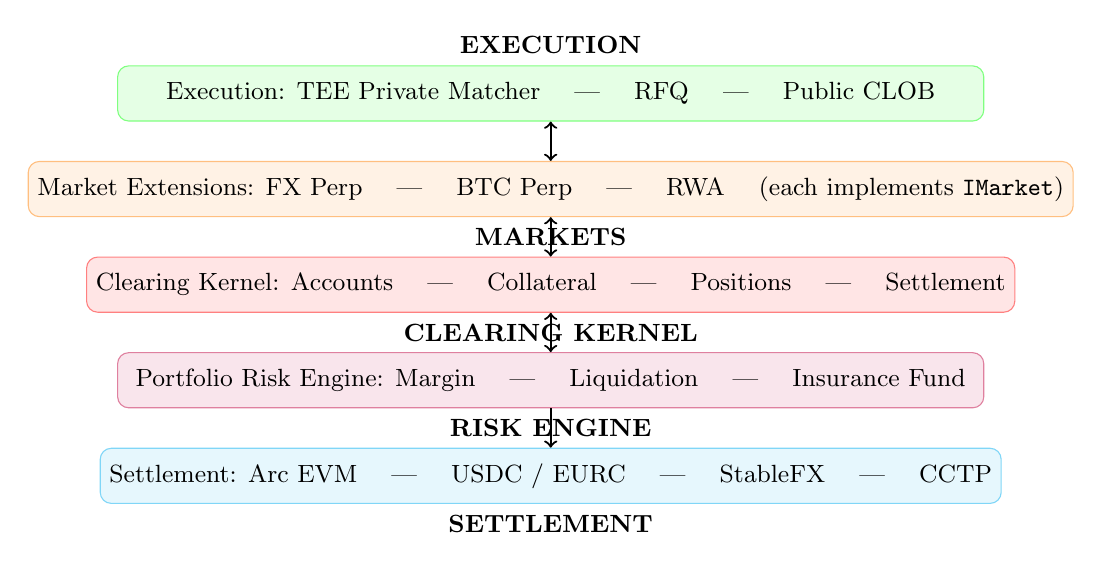
\begin{tikzpicture}[
    layer/.style={rectangle, draw, rounded corners, minimum width=11cm, minimum height=0.7cm, font=\small},
    exec/.style={layer, fill=green!10, draw=green!50},
    mkt/.style={layer, fill=orange!10, draw=orange!50},
    clear/.style={layer, fill=red!10, draw=red!50},
    risk/.style={layer, fill=purple!10, draw=purple!50},
    settle/.style={layer, fill=cyan!10, draw=cyan!50},
    label/.style={font=\small\bfseries, align=center}
  ]
    \node[exec] (execution) {Execution: TEE Private Matcher \quad | \quad RFQ \quad | \quad Public CLOB};
    \node[label, above=0.02cm of execution] {EXECUTION};

    \node[mkt, below=0.5cm of execution] (markets) {Market Extensions: FX Perp \quad | \quad BTC Perp \quad | \quad RWA \quad (each implements \texttt{IMarket})};
    \node[label, below=0.02cm of markets] {MARKETS};

    \node[clear, below=0.5cm of markets] (clearing) {Clearing Kernel: Accounts \quad | \quad Collateral \quad | \quad Positions \quad | \quad Settlement};
    \node[label, below=0.02cm of clearing] {CLEARING KERNEL};

    \node[risk, below=0.5cm of clearing] (risk) {Portfolio Risk Engine: Margin \quad | \quad Liquidation \quad | \quad Insurance Fund};
    \node[label, below=0.02cm of risk] {RISK ENGINE};

    \node[settle, below=0.5cm of risk] (settlement) {Settlement: Arc EVM \quad | \quad USDC / EURC \quad | \quad StableFX \quad | \quad CCTP};
    \node[label, below=0.02cm of settlement] {SETTLEMENT};

    \draw[<->, thick] (execution.south) -- (markets.north);
    \draw[<->, thick] (markets.south) -- (clearing.north);
    \draw[<->, thick] (clearing.south) -- (risk.north);
    \draw[->, thick] (risk.south) -- (settlement.north);
  \end{tikzpicture}
  \caption{Cerdic layers. Only settlement is one-directional -- everything above it can query and be queried.}
  \label{fig:architecture}
\end{figure}

Three rules govern the layering: (1) a market extension cannot touch kernel state except through the interface in Section~\ref{sec:markets}; (2) the kernel implements only accounting, collateral, and settlement -- nothing market-specific; (3) execution (matching) can be off-chain or TEE-based, but settlement is always a deterministic on-chain state transition.

%=============================================================================
\section{Clearing Kernel}
\label{sec:clearing}
%=============================================================================

\subsection{Account and collateral}

An account is a tuple $A = (\mathcal{B}, \mathcal{P}, \mathcal{H})$: collateral balances $\mathcal{B}$ by asset, an open position set $\mathcal{P}$ by market, and a credit/debit history $\mathcal{H}$.

\begin{table}[h]
  \centering
  \begin{tabular}{lll}
    \toprule
    \textbf{Tier} & \textbf{Assets} & \textbf{Haircut} \\
    \midrule
    1 & USDC, EURC & 0\% \\
    2 & USYC, stUSD & 2\%--5\% \\
    3 & ETH, BTC (liquid staking) & 10\%--20\% \\
    4 & Tokenized RWAs & 15\%--35\% \\
    \bottomrule
  \end{tabular}
  \caption{Collateral tiers. A cross-chain (CCTP) asset keeps its tier and adds a +2\%--5\% haircut for bridging latency.}
  \label{tab:collateral}
\end{table}

Effective collateral: $\mathcal{C}_{\text{eff}} = \sum_{a} b_a \cdot (1 - h_a) \cdot p_a$, summed over balance $b_a$, haircut $h_a$, and oracle price $p_a$.

\subsection{Trade lifecycle}

\begin{figure}[h]
  \centering
  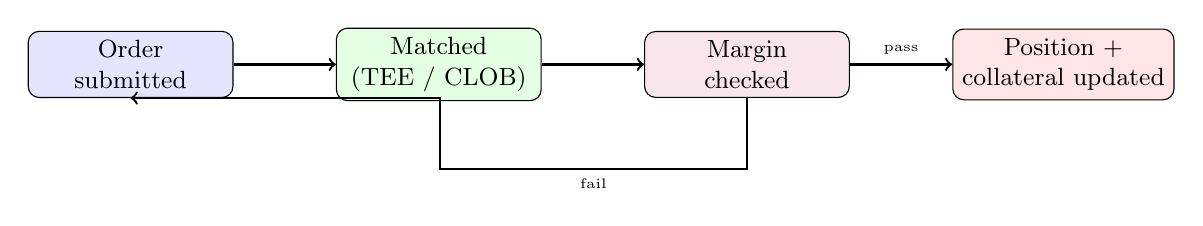
\begin{tikzpicture}[
    stepbox/.style={rectangle, draw, rounded corners, minimum width=2.6cm, minimum height=0.7cm, align=center, font=\small},
    arrow/.style={->, thick}
  ]
    \node[stepbox, fill=blue!10] (order) {Order\\submitted};
    \node[stepbox, fill=green!10, right=1.3cm of order] (match) {Matched\\(TEE / CLOB)};
    \node[stepbox, fill=purple!10, right=1.3cm of match] (check) {Margin\\checked};
    \node[stepbox, fill=red!10, right=1.3cm of check] (settle) {Position +\\collateral updated};

    \draw[arrow] (order) -- (match);
    \draw[arrow] (match) -- (check);
    \draw[arrow] (check) -- node[above, font=\tiny] {pass} (settle);
    \draw[arrow] (check.south) -- ++(0,-0.9) -- node[below, font=\tiny] {fail} ++(-3.9,0) |- (order.south);
  \end{tikzpicture}
  \caption{Every trade takes this path regardless of which market extension or execution mode produced the match.}
  \label{fig:lifecycle}
\end{figure}

Funding settlement and liquidation settlement follow the same shape: an event triggers a kernel-computed balance change, applied atomically with the position update. Positions are stored as opaque bytes with typed accessors -- the kernel does not interpret market-specific fields, it only enforces that collateral changes are atomic with position changes.

%=============================================================================
\section{Portfolio Margin}
\label{sec:margin}
%=============================================================================

Margining each position independently over-collateralizes hedged accounts. A trader long 10 BTC-notional on one market and short 9.5 BTC-notional on another has 0.5 BTC of real risk but would post margin on 19.5 BTC of gross notional under isolated margin. Cerdic margins the account, not the position.

\[
\mathcal{M}(\mathcal{P}) = f_S(\mathcal{P}) + f_C(\mathcal{P}) + f_L(\mathcal{P}) + f_K(\mathcal{P})
\]

\begin{itemize}
  \item $f_S$ -- \textbf{scenario margin}: worst-case loss across a scenario set $\mathcal{S}$ (parallel price shifts, funding-rate spikes, correlation breakdown): $f_S(\mathcal{P}) = \max_{s \in \mathcal{S}} \sum_{p \in \mathcal{P}} \big(V_p(s) - V_p(\text{current})\big)$.
  \item $f_C$ -- \textbf{concentration charge}: penalizes exposure concentrated in one asset group beyond a threshold $\theta$.
  \item $f_L$ -- \textbf{liquidity charge}: $\sum_p |\text{size}_p| \cdot \ell_p$, larger for thinner markets.
  \item $f_K$ -- \textbf{correlation adjustment}: for signed sizes $s_i, s_j$ and correlation $\rho_{ij}$, $f_K = \beta \sum_{i \neq j} \rho_{ij} \cdot s_i \cdot s_j$. Opposite-direction correlated positions ($s_i s_j < 0$) reduce margin -- a genuine hedge; same-direction correlated positions ($s_i s_j > 0$) increase it, since that is concentrated risk, not diversification. Sign matters: using unsigned sizes here would grant a margin discount to same-direction bets, which is wrong.
\end{itemize}

MVP ships two markets (Section~\ref{sec:roadmap}), but EURC/USDC and BTC/USDC are not economically correlated, so $f_C$/$f_K$ still have nothing meaningful to act on between them. $f_S$ and $f_L$ do real work from day one; $f_C$/$f_K$ become load-bearing once a second correlated market exists -- a second FX pair, or two accounts taking opposite sides of the same pair.

\subsection{Hedging is not a new feature}

A trader is "hedged," in this model, whenever they hold two correlated positions in opposite directions -- $f_K$ prices that automatically. Nothing extra needs to be built for a trader to hedge manually: open the offsetting position, watch $\mathcal{M}(\mathcal{P})$ drop. What \emph{is} new infrastructure is a strategy vault (Section~\ref{sec:yield}) automating that same offset on a rule set instead of a human clicking twice -- a sub-account with its own rebalance trigger, trading through the same kernel path as any other account. The margin math is identical either way; a vault only adds the automation layer on top of it.

\begin{figure}[h]
  \centering
  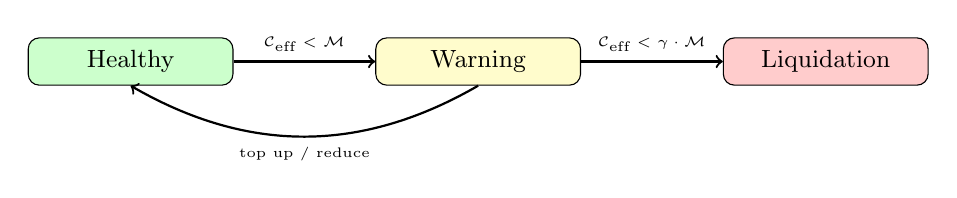
\begin{tikzpicture}[
    state/.style={rectangle, rounded corners, draw, minimum width=2.6cm, minimum height=0.6cm, align=center, font=\small},
    arrow/.style={->, thick}
  ]
    \node[state, fill=green!20] (healthy) {Healthy};
    \node[state, fill=yellow!20, right=1.8cm of healthy] (warning) {Warning};
    \node[state, fill=red!20, right=1.8cm of warning] (liq) {Liquidation};

    \draw[arrow] (healthy) -- node[above, font=\tiny] {$\mathcal{C}_{\text{eff}} < \mathcal{M}$} (warning);
    \draw[arrow] (warning) -- node[above, font=\tiny] {$\mathcal{C}_{\text{eff}} < \gamma \cdot \mathcal{M}$} (liq);
    \draw[arrow, bend left] (warning.south) to node[below, font=\tiny] {top up / reduce} (healthy.south);
  \end{tikzpicture}
  \caption{Liquidation state machine. $\gamma \approx 0.8$--$0.9$. Liquidation itself is tranched, not all-at-once, to avoid cascades (Section~\ref{sec:security}).}
  \label{fig:liquidation}
\end{figure}

The insurance fund target scales with the square root of aggregate squared position size, $F^* = \kappa\sqrt{\sum_p \text{size}_p^2}$, with $\kappa$ calibrated against historical stress periods before mainnet.

%=============================================================================
\section{Market Extensions}
\label{sec:markets}
%=============================================================================

A market extension implements one interface and a handful of lifecycle callbacks; the kernel never needs to know what the market \emph{is}.

\begin{figure}[h]
  \caption{\texttt{IMarket} (simplified)}
  \label{alg:market}
  \begin{quote}
  \texttt{\textbf{struct} MarketPosition \{ marketId, size (signed), entryPrice, margin, leverageCeiling \}} \\
  \texttt{getPnL(oraclePrice)} \quad \texttt{getFunding(position, period)} \\
  \texttt{validateOpen(size, collateral)} \quad \texttt{validateClose(position)} \\
  \texttt{onOpen / onClose / onLiquidate(user, market, position)}
  \end{quote}
\end{figure}

\texttt{leverageCeiling} is a per-market bound, not a trader's effective leverage -- because margin is computed at the account level (Section~\ref{sec:margin}), effective leverage is total notional over $\mathcal{C}_{\text{eff}}$, an account-level number the risk engine computes, not something read off one position.

\subsection{FX perpetual (first module)}

EURC/USDC at launch, additional pairs after. Funding follows the interest-rate differential, $r_{\text{FX}} = r_{\text{quote}} - r_{\text{base}}$. The spot leg of a settled trade can route through StableFX's PvP settlement rather than requiring Cerdic to bootstrap its own EURC/USDC liquidity. This is the module the rest of the paper's examples assume.

\subsection{Later modules (not required for the FX thesis, kept for continuity)}

A BTC/USDC perpetual proves the interface generalizes beyond FX. RWA and rate modules (tokenized Treasuries, USYC yield trading) and strategy vaults (delta-neutral, FX carry, funding arbitrage) follow the same interface once a second correlated market makes portfolio margin's $f_C$/$f_K$ terms meaningful. None of these require kernel changes to add.

%=============================================================================
\section{Private Matching}
\label{sec:privacy}
%=============================================================================

\begin{figure}[h]
  \centering
  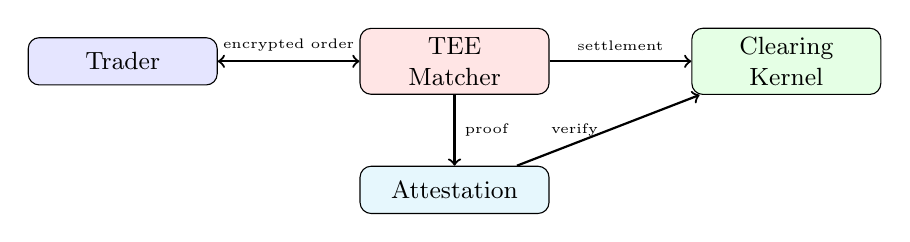
\begin{tikzpicture}[
    comp/.style={rectangle, draw, rounded corners, minimum width=2.4cm, minimum height=0.6cm, align=center, font=\small},
    arrow/.style={->, thick},
    doublearrow/.style={<->, thick}
  ]
    \node[comp, fill=blue!10] (user) {Trader};
    \node[comp, fill=red!10, right=1.8cm of user] (tee) {TEE\\Matcher};
    \node[comp, fill=green!10, right=1.8cm of tee] (kernel) {Clearing\\Kernel};
    \node[comp, fill=cyan!10, below=0.9cm of tee] (attest) {Attestation};

    \draw[doublearrow] (user) -- node[above, font=\tiny] {encrypted order} (tee);
    \draw[arrow] (tee) -- node[above, font=\tiny] {settlement} (kernel);
    \draw[arrow] (tee) -- node[right, font=\tiny] {proof} (attest);
    \draw[arrow] (attest) -- node[left, font=\tiny] {verify} (kernel);
  \end{tikzpicture}
  \caption{An order is only ever decrypted inside the enclave. The chain sees an attested settlement, never the order.}
  \label{fig:tee}
\end{figure}

The trader encrypts an order to the TEE's public key; the enclave decrypts, matches, and produces a signed attestation that on-chain verification checks before the settlement is accepted. If attestation fails, the system falls back to public settlement rather than blocking the trade. Verifying a TDX/SEV-SNP attestation directly on-chain costs roughly 75M gas; compressing it with a ZK proof of the attestation (following Kalypso's approach~\cite{marlin_kalypso}) brings that to roughly 300K gas -- a defense-in-depth layer over the TEE, not a replacement for it. Side-channel attacks on the enclave (cache timing, power analysis) are acknowledged and out of scope for the current design.

\subsection{On-chain footprint of a private position}
\label{sec:sealed}

Matching an order privately is only half the claim -- the position that results has to stay private too, or the TEE only hid the five seconds before a trade. Cerdic keeps two things off-chain in plaintext:

\begin{itemize}
  \item \textbf{Sealed position parameters.} Side, leverage, entry price, size, and any TP/SL thresholds are never stored as separate on-chain fields. They are collapsed into one \texttt{sealedParams: bytes} blob, encrypted to the TEE's key, alongside a plain \texttt{collateral} amount and \texttt{status} the kernel needs for solvency accounting. Any check that would otherwise read a plaintext field -- a TP/SL trigger, a liquidation solvency check, a margin recomputation -- runs \emph{inside} the enclave against the decrypted blob; the contract never re-derives it from public state.
  \item \textbf{Portfolio linkage.} Cross-margined positions are grouped by a \texttt{portfolioKey} -- a hash the TEE derives from the account's private key material, not the account address itself. The risk engine still sees the full position set behind a \texttt{portfolioKey} when it computes $\mathcal{M}(\mathcal{P})$ (Section~\ref{sec:margin}), because it has to; an outside observer sees only that some set of positions shares a key, not whose account that is or what the set contains.
\end{itemize}

The kernel authorizes exactly one caller -- the attested TEE -- to invoke settlement, liquidation, and TP/SL-trigger functions. It does not recompute PnL or check thresholds against plaintext; it checks that the caller is the attested TEE and that its own invariants hold (collateral bounds, no double-settlement), then applies the number the TEE provides. This means events can be stripped to the minimum needed for indexing:

\begin{table}[h]
  \centering
  \begin{tabular}{ll}
    \toprule
    \textbf{Event} & \textbf{Emits} \\
    \midrule
    Position opened & \texttt{positionId}, \texttt{collateral} \\
    Position closed / liquidated & \texttt{positionId} only \\
    Trade settled & \texttt{matchId} only \\
    \bottomrule
  \end{tabular}
  \caption{No event carries price, size, side, or PnL. Oracle price and settlement amount are consumed by the kernel from the TEE's authenticated call, not re-emitted.}
  \label{tab:events}
\end{table}

This is deliberately not full position-level ZK privacy (commitment/nullifier circuits proving position validity without any party but the trader ever seeing the plaintext, as in comparable Stellar-based designs). That is a stronger, ZK-native version of the same idea, and a heavier build; sealed params plus an authorized-settler contract gets most of the same on-chain opacity with Solidity and a TEE, no circuit design required, and composes cleanly with the ZK layer already on Cerdic's roadmap (Section~\ref{sec:roadmap}) if solvency-proof-style privacy is needed later.

Two other execution modes exist for markets that do not need this: a \textbf{public CLOB} for transparent price discovery, and \textbf{RFQ} for block trades where a taker requests quotes and settles atomically against the best one.

\subsection{Why this is not an on-chain order book}

The TEE matcher keeps full order-book semantics -- continuous matching, price-time priority, standing orders -- but the book itself lives in enclave memory, not contract storage; the chain only sees attested settlements. A literal on-chain order book with privacy (order state encrypted in contract storage, matched by FHE or a ZK circuit without ever decrypting) is a harder, still-immature problem: continuous FHE compute per match is expensive today, and putting per-order state on-chain works directly against Section~\ref{sec:margin}'s cost profile, where the expensive operation is already the full-portfolio margin recomputation, not order placement. TEE matching gets the useful property -- a private, continuously-matched book -- without inheriting that cost. A ZK-proved batch auction (commitments on-chain, a proof that the clearing price was computed correctly, no plaintext order ever posted) is the more realistic next privacy-preserving execution mode, and is already covered by the batch-verification proof in Section~\ref{sec:security}'s ZK layer -- it is a variant of an existing roadmap item, not a new one.

%=============================================================================
\section{Agents}
\label{sec:agents}
%=============================================================================

An agent account is a normal clearing account with a cryptographic identity and a scoped, signed capability instead of a human signer behind every action:

\[
\text{capability} = \text{Sign}_{sk_{\text{owner}}}\big(H(\text{agent\_id}, \text{action}, \text{limits}, \text{expiry})\big)
\]

The kernel checks the owner's signature before honoring any action under the capability. Execution policy (max position size, max leverage, daily loss limit, allowed markets) is enforced at the kernel level, not trusted to the agent's own code. Session keys are ephemeral and scoped, so an agent never needs the owner's master key. High-frequency agent-to-agent transfers (data fees, per-call payments) use Circle's Nanopayments so sub-cent transfers stay economical~\cite{circle_nanopayments}, and agent identity is designed to be compatible with Circle's Agent Stack~\cite{circle_agent_stack}.

%=============================================================================
\section{Yield}
\label{sec:yield}
%=============================================================================

Collateral tiers (Table~\ref{tab:collateral}) are not just haircut buckets -- each accrues yield to the depositor while still counting toward margin. USDC/EURC can sweep into overnight repo; USYC carries its own money-market yield~\cite{usyc}; RWA collateral earns its underlying's yield at a wider haircut. Yield accrual never reduces an asset's margin eligibility -- value for margin purposes is market value plus accrued yield.

Strategy vaults are the same mechanism at the account level: a vault is a sub-account with its own risk isolation, trading through the same kernel and margined the same way as any trader, so a vault-specific strategy failure cannot leak into other accounts. This is also how CLOB/RFQ liquidity gets provided -- market-making is one more vault strategy, not a separate pooled-liquidity system with its own risk model.

%=============================================================================
\section{Economics}
\label{sec:economics}
%=============================================================================

No protocol token. Every incentive is paid in stablecoins or yield-bearing assets, which keeps regulatory treatment simple and avoids emissions-driven liquidity that has to be unwound later.

\begin{table}[h]
  \centering
  \begin{tabular}{lll}
    \toprule
    \textbf{Fee} & \textbf{Rate} & \textbf{Goes to} \\
    \midrule
    Taker & 0.03\%--0.06\% & LPs, treasury \\
    Maker & 0\%--0.02\% & LPs \\
    Vault performance & 10\%--20\% & Vault manager, treasury \\
    Yield keep & 0\%--10 bps & Treasury \\
    Liquidation penalty & 1\%--5\% & Liquidator, insurance fund \\
    \bottomrule
  \end{tabular}
  \caption{Fee schedule. Dynamic within these ranges by volume tier.}
  \label{tab:fees}
\end{table}

The tradeoff of no token: early liquidity has to be earned with real fee yield and USYC-denominated incentives from the treasury rather than bootstrapped with emissions, which is slower but does not need to be unwound later.

%=============================================================================
\section{Security}
\label{sec:security}
%=============================================================================

\begin{description}
  \item[Oracles] Pyth (primary), Chainlink (staleness check), CLOB TWAP (circuit-breaker reference). A $\delta$ divergence (1\%--5\%) between primary and secondary pauses the affected market.
  \item[Liquidation cascades] Positions are liquidated in tranches, ordered by time-in-distress, with a volume-based circuit breaker if total liquidation flow in a window exceeds a threshold.
  \item[Kernel invariants] Collateral cannot be created or destroyed outside authorized operations; position and collateral updates are atomic; settlement is deterministic given the same input state; a market extension cannot touch kernel state outside its interface.
  \item[TEE] Compromise leaks order flow, not funds -- settlement correctness never depends on the enclave, only confidentiality does.
\end{description}

%=============================================================================
\section{Roadmap}
\label{sec:roadmap}
%=============================================================================

\subsection{MVP: private, portfolio-margined EURC/USDC (and BTC/USDC) perpetuals}

Every component below is real and working end-to-end, not a stub -- the point of the MVP is proving all three pillars together, not demoing them separately.

\begin{itemize}
  \item Clearing kernel (Solidity, Arc EVM, Foundry): accounts, collateral, positions, settlement.
  \item One FX market extension (EURC/USDC) plus the existing BTC/USDC extension, both against the same \texttt{IMarket} interface.
  \item Full portfolio margin engine ($f_S+f_C+f_L+f_K$), on-chain enforced, off-chain computed.
  \item TEE-matched private RFQ against a real enclave (GCP Confidential Space, AMD SEV-SNP), with on-chain attestation verification and public-settlement fallback.
  \item Agent accounts: identity, capability tokens, session keys, one working agent type (trading agent), Nanopayments-integrated.
  \item USYC as a live collateral tier.
  \item Frontend (Next.js) via Circle Developer Controlled Wallets; Arc Testnet deployment.
\end{itemize}

\subsection{Phase 1 -- hardening}
Formal verification of kernel and margin invariants; wider scenario coverage in $f_S$ (vol shocks, correlation-breakdown regimes); additional crypto markets; multi-asset collateral with dynamic haircuts; mainnet.

\subsection{Phase 2 -- more markets}
Additional FX pairs (GBP/USD, JPY/USD); RWA and rate module; strategy vaults; internal repo market; CCTP v2 cross-chain collateral.

\subsection{Phase 3 -- scale}
ZK solvency attestation for institutions; ZK-compressed TEE attestation verification; institutional sub-accounts; agent strategy vaults (smart treasuries); migration path to Arc's protocol-level privacy roadmap (APS) if and when it ships.

%=============================================================================
\section{Conclusion}
\label{sec:conclusion}
%=============================================================================

Arc settles stablecoin value. StableFX settles spot FX conversion on top of it. Neither gives a trader leverage, and neither hides an order before it executes. Cerdic is the layer that does both: post collateral once, get portfolio-margined leverage across correlated positions, match privately through a TEE, settle through the same rails Circle already built. Ostium already proved leveraged onchain FX/RWA has demand; Cerdic's bet is that the next version of that market is private and portfolio-margined, on the chain built specifically for stablecoin-native FX.

\paragraph{Acknowledgements.} We thank the Circle Arc and Encode Club communities for the accelerator context that motivated this work.

\bibliographystyle{plain}
\bibliography{references}

\end{document}
